\section{Results}
\label{sec:results}
\begin{table}[t]
\centering
\caption{Main result: Spearman correlation between model similarity $S^{\mathrm{emb}}$ and $-D$, averaged over the three IC families (153 pairs each). Samples 0--9, with the reference computed on the same samples. Brackets: 95\% bootstrap intervals. Baseline values in parentheses use all 100 samples.}
\label{tab:main}
\small
\setlength{\tabcolsep}{3.5pt}
\resizebox{\columnwidth}{!}{%
\begin{tabular}{lccc}
\toprule
Model & Text & Image & Joint \\
\midrule
EmbeddingGemma 2 & 0.21 {\scriptsize[0.21, 0.23]} & 0.76 {\scriptsize[0.73, 0.79]} & 0.23 {\scriptsize[0.22, 0.24]} \\
Qwen3-VL-Emb.-2B & 0.44 {\scriptsize[0.39, 0.45]} & 0.78 {\scriptsize[0.73, 0.83]} & 0.39 {\scriptsize[0.35, 0.40]} \\
GME-Qwen2-VL-2B & 0.46 {\scriptsize[0.44, 0.47]} & 0.83 {\scriptsize[0.75, 0.84]} & 0.50 {\scriptsize[0.47, 0.54]} \\
\midrule
Char.\ TF--IDF (text) & 0.35 {\scriptsize(0.36)} & -- & -- \\
Rendered pixels (image) & -- & 0.93 {\scriptsize(0.95)} & -- \\
Fourier magnitudes (image) & -- & 0.44 {\scriptsize(0.42)} & -- \\
Initial frame only (image) & -- & undefined & -- \\
\bottomrule
\end{tabular}}
\end{table}


\begin{figure*}[t]
\centering
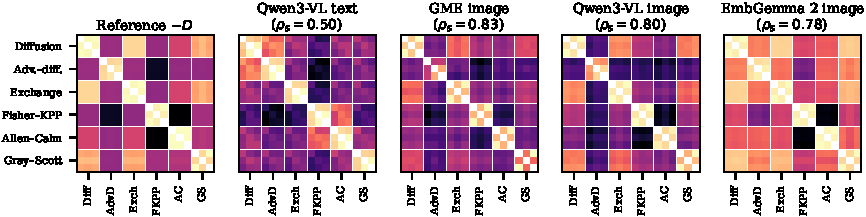
\includegraphics[width=\textwidth]{figures/fig_matrices.pdf}
\caption{Similarity between the 18 problems of the oscillation family (samples 0--9). Rows and columns are grouped by equation, with the periodic, Dirichlet, and Neumann versions inside each block. Brighter means more similar; the diagonal is left blank, and each panel has its own color scale. $\rho_s$ is the Spearman correlation with $-D$ for this family. Every model sees that the three BC versions of an equation are nearly the same. The image embeddings also recover much of the structure between equations; the text embedding recovers less of it.}
\label{fig:matrices}
\end{figure*}

\subsection{Main Results}
\paragraph{Images work best, but not better than pixels.}
With images, the three models reach Spearman correlations of \spImageMin--\spImageMax{} with the reference and triplet accuracies of \trImageMin--\trImageMax{} (\cref{tab:main,tab:secondary,fig:matrices}). That is real agreement. But every model falls short of simply comparing the pixels (\spPix{}), and lands close to the physical cosine (\spPhys{}), which ignores how strong a response is. For Qwen3-VL and GME, the image similarities actually follow the physical cosine more closely (Spearman \spQwImagePhys{} and \spGmeImagePhys{}) than they follow the reference. EmbeddingGemma 2 does not show this pattern (\spGemImagePhys{}). On this benchmark, the pretrained image features add nothing to the ranking that the pixels do not already contain, and they partly lose the size of the response.

\paragraph{Text descriptions agree only weakly.}
With text, the correlations are \spTextMin--\spTextMax{}. Qwen3-VL (\spQwText{}) and GME (\spGmeText{}) beat character TF--IDF (\spTfidf{}) by a small margin, and EmbeddingGemma 2 (\spGemText{}) does worse than it. All three models give the highest similarity to descriptions that share an equation (\cref{tab:factors}), which matches the reference. They do much worse at ordering different equations. On pairs with the same BC, where only the equation changes, the correlations are \spQwTextSame{}, \spGmeTextSame{}, and \spGemTextSame{}. In other words, the text embeddings recognize when two problems use the same equation, but they say little about how far apart the solutions of two different equations will end up.

\paragraph{Adding the image to the text helps little.}
With both inputs, the correlations are \spBothMin--\spBothMax{}. Each model stays close to its text-only score and far below its image-only score. Only GME improves noticeably over text alone (\spGmeBoth{} against \spGmeText{}). In every model, the description uses more tokens than the image (\cref{tab:model-inputs}). The mismatch control below shows that the models weigh the two inputs differently.

\paragraph{Other references.}
The image results hold up against the 100-frame reference (\spQwImageHund{}, \spGmeImageHund{}, and \spGemImageHund{} for Qwen3-VL, GME, and EmbeddingGemma 2) and across all 54 problems, where differences in the initial data also enter (\spQwImageFull{}, \spGmeImageFull{}, \spGemImageFull{}). Across all 54 problems, the text embeddings (\spQwTextFull{}, \spGmeTextFull{}, \spGemTextFull{}) fall far behind character TF--IDF (\spTfidfFull{}), which picks up the different IC formulas. Since every triplet is reliable, accuracy on reliable triplets equals overall accuracy, and triplets made only of linear equations show the same pattern (\cref{tab:secondary}).

\subsection{Controls}
\Cref{tab:controls} summarizes the controls. Encoding the same initial-frame image twice gave bit-identical embeddings in every model, so that control indeed has constant scores.

\paragraph{Time order.}
Reversing the snapshots hardly changes how well the image similarities match the reference (samples 0--2, original/reversed: \revOrigQw{}/\revRevQw{}, \revOrigGme{}/\revRevGme{}, and \revOrigGem{}/\revRevGem{} for Qwen3-VL, GME, and EmbeddingGemma 2). This is expected, since the reference does not depend on frame order. Yet the reversal moves each image embedding a long way. For Qwen3-VL and GME, an image and its reversed copy are about as similar (\revSelfQw{} and \revSelfGme{}) as the two least similar problems in an IC family (\rangeLoQwImage{} and \rangeLoGmeImage{}). For EmbeddingGemma 2 the value (\revSelfGem{}) lies inside that range. The models notice the layout, but nothing suggests that they use the direction of time.

\paragraph{Notation.}
Rewriting a description in equivalent notation changes its embedding a great deal. On average, an original description is more similar to its nearest \emph{different} problem (\notOtherQw{}, \notOtherGme{}, and \notOtherGem{} for Qwen3-VL, GME, and EmbeddingGemma 2) than to its own rewrite (\notSelfQw{}, \notSelfGme{}, and \notSelfGem{}). For GME and EmbeddingGemma 2 the effect is extreme: for \notAllGme{} and \notAllGem{} of descriptions, all 53 other problems, including those with different equations and different initial data, are closer to the original than its rewrite is. For Qwen3-VL, a median of \notCloserQw{} of the 53 are closer. Seen from the other side, a rewrite still finds its own original among the 54 descriptions of its sample in \notTopQw{}, \notTopGme{}, and \notTopGem{} of cases. The rewrite moves the embedding to a new region, not onto another problem. The rewritten descriptions match the reference no better than the originals (Spearman \notSpQw{}, \notSpGme{}, and \notSpGem{}, against \notSpOrigQw{}, \notSpOrigGme{}, and \notSpOrigGem{} on the same samples).

\paragraph{Mismatched inputs.}
When the image and the description disagree, Qwen3-VL follows the description: its joint similarities match the reference of the described problem (\misDeckQw{}) rather than the problem shown (\misImgQw{}). GME weighs the two about equally (\misDeckGme{} and \misImgGme{}), and EmbeddingGemma 2 leans toward the image (\misDeckGem{} and \misImgGem{}), even though its matched joint input does no better than text alone. So the image does reach the joint embedding, but in no model does it lift the joint score close to the image-only score.

\paragraph{Changing one coefficient.}
In the heat-equation test, where the four descriptions differ only in the diffusion coefficient, Qwen3-VL and EmbeddingGemma 2 rank the candidates in the correct order, $S(0.01,0.011)>S(0.01,0.02)>S(0.01,0.05)$. GME reverses it (similarities \heatValsGme{}).

\begin{table*}[t]
\centering
\caption{Further results on samples 0--9, averaged over IC families. Triplet accuracy for all triplets, for triplets whose order is guaranteed despite numerical error (``reliable''), and for triplets made only of linear equations, where the guarantee is exact. Spearman correlation for pairs with the same BC (45 per family) and with different BCs (108 per family), against the 100-frame reference, and over all 1,431 pairs of the 54 problems.}
\label{tab:secondary}
\small
\begin{tabular}{llccccccc}
\toprule
& & \multicolumn{3}{c}{Triplet accuracy} & \multicolumn{2}{c}{Spearman by BC} & \multicolumn{2}{c}{Spearman, other references} \\
\cmidrule(lr){3-5}\cmidrule(lr){6-7}\cmidrule(lr){8-9}
Model & Input & All & Reliable & Linear & Same BC & Diff.\ BC & 100 frames & All 54 \\
\midrule
EmbeddingGemma 2 & text & 0.57 & 0.57 & 0.70 & $-$0.26 & 0.32 & 0.24 & 0.28 \\
 & image & 0.78 & 0.78 & 0.79 & 0.64 & 0.80 & 0.70 & 0.83 \\
 & joint & 0.58 & 0.58 & 0.70 & $-$0.09 & 0.33 & 0.25 & 0.39 \\
Qwen3-VL-Emb.-2B & text & 0.65 & 0.65 & 0.66 & 0.22 & 0.53 & 0.36 & 0.20 \\
 & image & 0.79 & 0.79 & 0.83 & 0.69 & 0.82 & 0.88 & 0.77 \\
 & joint & 0.66 & 0.66 & 0.65 & 0.11 & 0.49 & 0.34 & 0.22 \\
GME-Qwen2-VL-2B & text & 0.64 & 0.64 & 0.69 & 0.18 & 0.55 & 0.49 & 0.29 \\
 & image & 0.84 & 0.84 & 0.87 & 0.74 & 0.86 & 0.87 & 0.74 \\
 & joint & 0.67 & 0.67 & 0.76 & 0.26 & 0.59 & 0.54 & 0.53 \\
TF--IDF & -- & 0.61 & 0.61 & 0.71 & 0.26 & 0.48 & -- & 0.67 \\
Pixels & -- & 0.95 & 0.95 & 0.96 & 0.90 & 0.94 & -- & 0.99 \\
Fourier & -- & 0.73 & 0.73 & 0.57 & 0.20 & 0.52 & -- & 0.40 \\
Phys.\ cosine & -- & 0.90 & 0.90 & 0.98 & 0.74 & 0.85 & -- & 0.64 \\
\bottomrule
\end{tabular}
\end{table*}

\begin{table*}[t]
\centering
\caption{Controls on samples 0--2 (heat test: four short descriptions). Time order: Spearman correlation with $-D$ for original/reversed images, and the average similarity between an image and its reversed copy. Notation: how often a rewritten description finds its own original among the 54 descriptions of its sample (top-1), and the average similarity of an original to its rewrite/to its most similar other problem. Mismatch: Spearman correlation of joint embeddings (image of one problem, description of the next equation) with the image's reference/the description's reference. Heat: whether $S(0.01,0.011)>S(0.01,0.02)>S(0.01,0.05)$ with text input.}
\label{tab:controls}
\small
\begin{tabular}{lcccccc}
\toprule
& \multicolumn{2}{c}{Time order (image)} & \multicolumn{2}{c}{Notation (text)} & Mismatch (joint) & Heat \\
\cmidrule(lr){2-3}\cmidrule(lr){4-5}
Model & Orig./rev. & Self-sim. & Top-1 & Rewrite/other & Image/text ref. & order \\
\midrule
EmbeddingGemma 2 & 0.75/0.81 & 0.999 & 0.38 & 0.973/0.998 & 0.41/0.19 & yes \\
Qwen3-VL-Emb.-2B & 0.70/0.74 & 0.988 & 0.77 & 0.956/0.995 & 0.09/0.36 & yes \\
GME-Qwen2-VL-2B & 0.77/0.74 & 0.985 & 0.50 & 0.958/0.997 & 0.41/0.40 & no \\
\bottomrule
\end{tabular}
\end{table*}

